% !TeX spellcheck = hu_HU
\documentclass[12pt,a4paper]{article}
\usepackage[utf8]{inputenc}
\usepackage{cmap}
\usepackage[T1]{fontenc}
\usepackage[magyar]{babel}
\usepackage{amsmath}
\usepackage{amsfonts}
\usepackage{amssymb}
\usepackage{graphicx}

\usepackage{struktex}
\usepackage{outlines}
\usepackage{hyperref}

\hyphenpenalty=10000

%TeXstudio doesn't like leadsto by default
\renewcommand{\leadsto}{\rightsquigarrow}

\begin{document}

\begin{center}
	\huge
	Algoritmusok és adatszerkezetek II\\
	\vspace{1mm}
	\LARGE
	Mintaillesztés témakör jegyzete\\
	\vspace{5mm}
	\large
	Készült Ásványi Tibor előadásai és gyakorlatai alapján\\
	\vspace{5mm}
	Sárközi Gergő, 2021-22-1. félév\\
	Nincsen lektorálva!
\end{center}

\tableofcontents

\pagebreak

\section{Mintaillesztés}

\begin{outline}
	\1 Abécé: $\Sigma = \{\sigma_1, \sigma_2, ..., \sigma_d\}$ \;\; ($1 \le d < \infty$ konstans)
	\1 Szöveg, amiben keresünk: $T/1: \Sigma[n]$ \;\; ($1 \le n$)
	\1 Minta, amit keresünk: $P/1: \Sigma[m]$ \;\; ($1 \le m \le n$)
	\1 $s \in 0..(n-m)$ $P$ érvényes eltolása $T$-n $\Leftrightarrow T[s+1..s+m] = P[1..m]$
	\1 A cél az érvényes eltolások $S$ halmazának megállapítása
\end{outline}

\section{Egyszerű (brute force) algoritmus}

\begin{outline}
	\1 Minden lehetséges $s$ értékre, egymástól függetlenül, próbáljuk a mintát
	\1 Időkomplexitás: $MT(n,m) \in \Theta(n*m)$ és $mT(n,m) \in \Theta(n)$
		\2 Alapból $MT \in \Theta((n-m+1)*m)$ és $mT \in \Theta(n-m+1)$
		\2 $m \le n \implies (n-m+1) \in \Theta(n)$
		\2 Tehát $MT \in \Theta(n*m)$ és $mT \in \Theta(n)$ \;\;(mint legfelül)
		\2 Ha $m$ nem elhanyagolható $n$-hez képest ($m \ge \epsilon * n$ ahol $0 < \epsilon < 1$)\\
		akkor $(n*m) \in \Theta(n^2) \implies MT \in \Theta(n^2)$
\end{outline}

\begin{figure}[h!]
	\centering
	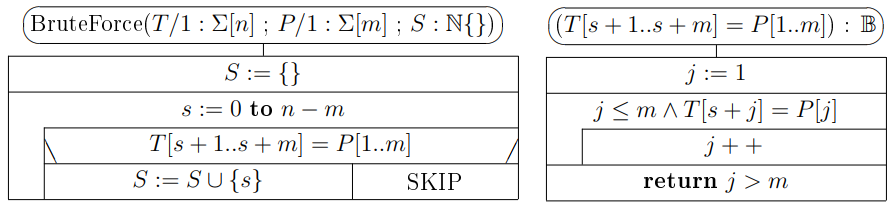
\includegraphics[width=0.95\linewidth]{BruteForce}
\end{figure}

\pagebreak

\section{Quicksearch}

\begin{outline}
	\1 Egynél nagyobb lépésekben növeli az $s$ eltolását (de nem ugrik át egy érvényes eltolást sem)
	\1 Előkészítő fázis: Ábécé minden $\sigma$ eleméhez $shift(\sigma) \in 1..m+1$ címke
		\2 Csak a mintától függ, a szövegtől nem
	\1 $shift(\sigma)$ működése:
		\2 $\sigma$ mindig a minta utáni első karakter a szövegben: $\sigma = T[s+m+1]$
		\2 Megmondja $T[s+1..s+m]$ megnézése után mennyivel nőjön $s$
		\2 Ha $\sigma \in P$: $s$ mennyivel nőjön, hogy a minta illeszkedhessen a $T[s+m+1]$ karakterre (pl. ha $P[m]=\sigma$ akkor $shift(\sigma)=1$)
		\2 Ha $\sigma \notin P$: minta átugorja $T[s+m+1]$ karaktert ($shift(\sigma) = m+1$)
	\1 Időkomplexitás:
		\2 $mT \in \Theta(\frac{n}{m+1}+m)$ (pl. $T$ és $P$ diszjunktak)
			\3 Jobb, mint a brute force megoldás
		\2 $MT \in \Theta((n-m+2)*m)$ (pl. $T$ és $P$ mind azonos $\sigma$ sokszor)
			\3 Azonos brute force-szal, de gyakorlatban lassabb
		\2 Átlagosan gyorsabb, mint a brute force, de azért nem optimális
\end{outline}

\begin{figure}[h!]
	\centering
	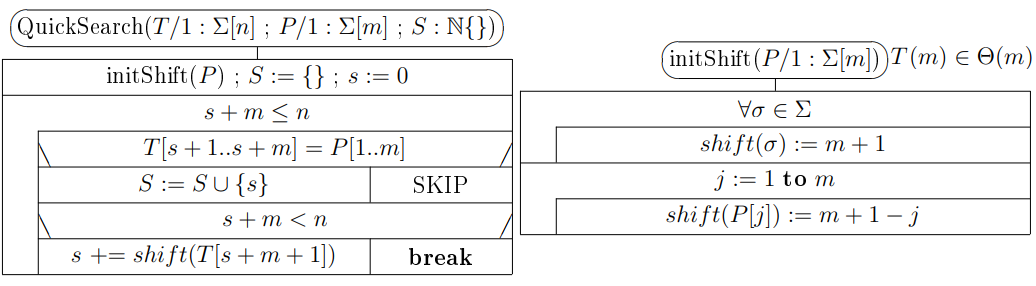
\includegraphics[width=1\linewidth]{QuickSearch}
\end{figure}

\pagebreak

\subsection{Quicksearch példa}

\begin{outline}
	\1 Bal fenti ábra:
		\2 $xxxx$ jelöli a mintával az eltolás előtt összehasonlított szövegrészt
		\2 Az eltolás mértékét mutatja be: az eltolás utána állapot látható
\end{outline}

\begin{figure}[h!]
	\centering
	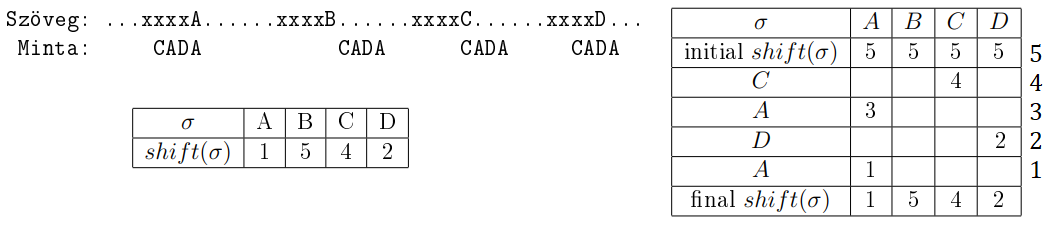
\includegraphics[width=1\linewidth]{QuickSearch-példa-shift}
\end{figure}

\begin{figure}[h!]
	\centering
	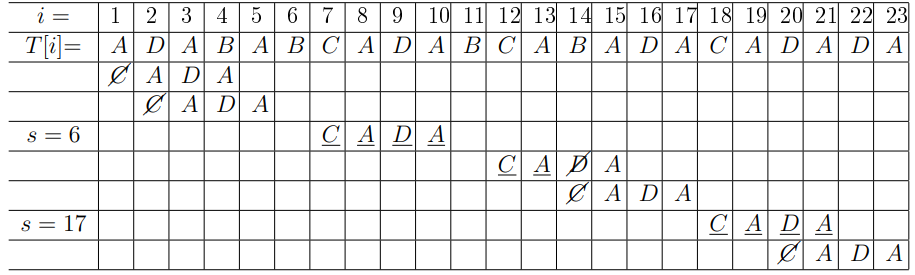
\includegraphics[width=1\linewidth]{QuickSearch-példa-táblázat}
\end{figure}

\pagebreak

\section{Knuth-Morris-Pratt (lineáris) algoritmus RÖVIDEN}

\begin{outline}
	\1 Lineáris időben végzi el a feladatot
	\1 Nem kell minden esetben a minta elejétől kezdeni az illesztést:\\
	a prefixet nem kell újra vizsgálni, ha az egyezik a szufixszel
	\1 Előfeldogozás: ($\Theta(m)$ idő alatt végbemegy)
		\2 megadunk egy $next$ függvényt, ami megadja a leghosszabb megegyező prefix-szuffix párok hosszát minden minta kezdőszeletre (hosszra)
		\2 $next(j)$ a leghosszabb olyan $P$ prefix hossza, amely $P$ első $j$ karakterének szuffixe (de nem egyezik meg vele), azaz $next(j) \in 0..(j-1)$
	\1 A szövegben nem kell visszaugrani, azaz buffer nélkül is használható.
	(Minden karaktert csak egyszer olvasunk ki, és csak "előrefelé" haladunk.)
	\1 A mintát sikeres/sikertelen illesztés esetén annyival toljuk előrebb,
	amerkkora a sikeresen illesztet részminta hossza MÍNUSZ
	a sikeresen illesztet részminta legnagyobb szuffixe, ami egyben prefix.\\
	Azaz ez a legnagyobb szuffix lesz a minta kezdete.
	\1 Időkomplexitás: $MT = mT \in \Theta(n)$
		\2 $\Omega(n)$, mert $i$ egyesével nő és $n$-ig megy
		\2 $O(n)$, $2i-j$ értéke mindig szig. mon. nő, tehát max $2n$ iteráció
\end{outline}

\begin{figure}[h!]
	\centering
	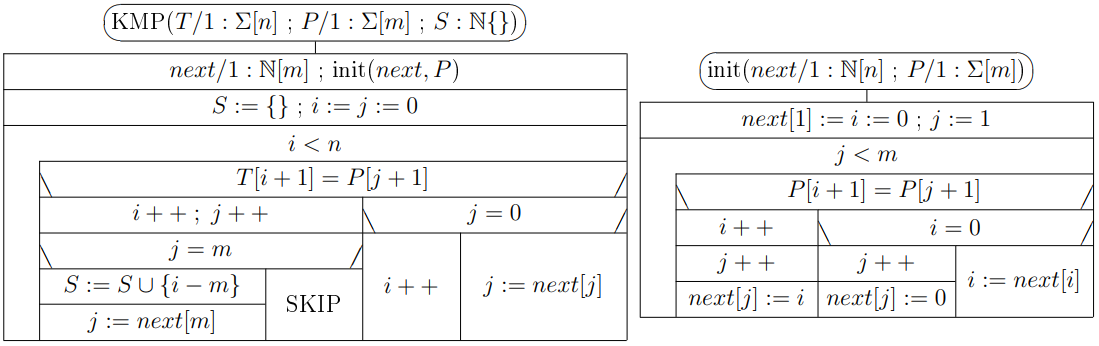
\includegraphics[width=1\linewidth]{KMP}
\end{figure}

\begin{outline}
	\1 $next[1]=0$
	\1 $next[i+1] \le next[i]+1$
	\1 $next(j) \in 0..(j-1) \;\; (j \in 1..m)$
\end{outline}

\pagebreak

\begin{outline}
	\1 $init$ ciklusának invariánsa:
		\2 $i \le j \le m$
		\2 $P$ első $i$ karaktere szuffixe $P$ első $j$ karakterének
		\2 és $\forall l \in (i+2)..j:$ $P$ első $l$ karaktere nem szuffixe $P$ első $j+1$ karakterének, de egyenlőek lehetnek
		\2 és $next[1..j] = next(1..j)$ (azaz a tömb a fv alapján van töltve)
	\1 $KMP$ ciklusának invariánsa:
		\2 $i \in 0..n$ és $j \in 0..(m-1)$ és $j \le i$
		\2 és $S = \{ s \in 0..(i-m) \;|\; T[(s+1)..(s+m)] = P \}$
		\2 és $P$ első $j$ karaktere szuffixe $T$ első i karakterének (vagy egyenlőek)
		\2 és $\forall l \in (j+2)..m:$ $P$ első $l$ karaktere nem szuffixe $T$ első $i+1$ karakterének (és nem is egyenlőek)
\end{outline}

\subsection{Példa}

\begin{figure}[h!]
	\centering
	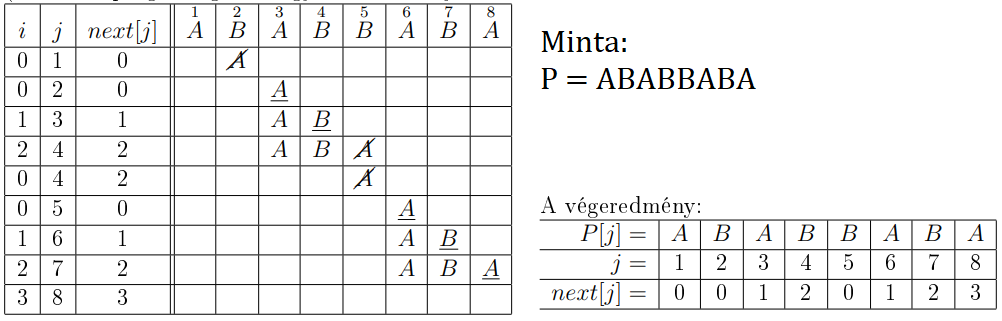
\includegraphics[width=1\linewidth]{KMP-példa-init}
\end{figure}

\begin{figure}[h!]
	\centering
	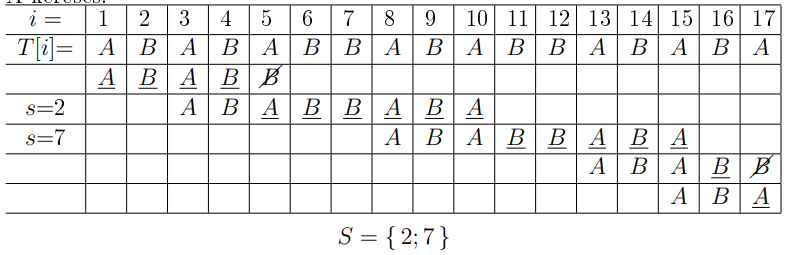
\includegraphics[width=1\linewidth]{KMP-példa-kmp}
\end{figure}

\pagebreak

\section{Knuth-Morris-Pratt (lineáris) algoritmus}

\subsection{Jelölések}

\begin{outline}
	\1 Akár teljes prefix: $x \sqsubseteq y \Leftrightarrow \exists z: x + z = y$
	\1 Igazi prefix: $x \sqsubset y \Leftrightarrow x \sqsubseteq y \wedge x \ne y$
	\1 Akár teljes szuffix: $x \sqsupseteq y \Leftrightarrow \exists z: z + x = y$
	\1 Igazi szuffix: $x \sqsupset y \Leftrightarrow x \sqsupseteq y \wedge x \ne y$
	\1 Az üres sztring mindennek a prefixe és a szuffixe is.
	\1 Kezdőszelet: $A_j = A[1..j]$ (ezt a jelölést ritkán használjuk)
		\2 $A_0$ az üres sztring
	\1 Prefix-szuffix: $x \square y \leftrightarrow x \sqsubset y \wedge x \sqsupset y$
	\1 $i.$ legnagyobb elem: $\max_i H$ \;\; ($i \in 1..|H|$)
		\2 $\max_1 H = \max H$ és $\max_{|H|} H = \min H$
	\1 $H(j) = \{h \in 0..j-1 \;|\; P_h \sqsupset P_j\} = \{|x| \;|\; x \square P_j\}$
	\;\; ($j \in 1..m$) \\
	Azaz azon sztring hosszak, amelyek prefixek és szuffixek is $P$-nek egyben.
	\1 $next(j) = \max H(j)$ \;\; ($j \in 1..m$)\\
	Leghosszab $P$-beli prefix hossza, ami egyben valódi szuffixe $P_j$-nek.
\end{outline}

NINCS BEFEJEZVE, NAGYON HIÁNYOS

\end{document}
